% SC4053 --- Chapter 6: Scaling (Channels, Rollups, Sharding) (0->100)
\chapter{Scaling: Channels, Rollups and Sharding}\label{ch:scaling}

\begin{quote}
\emph{``You cannot have a single machine do all the world's transactions without making it a centralised supercomputer. Scaling is about doing less on the bottleneck and proving it was done right.''} --- This chapter shows how.
\end{quote}

\noindent\fbox{\parbox{\dimexpr\linewidth-2\fboxsep-2\fboxrule}{%
\textbf{From zero: no scaling background assumed.} We start from a cafe tab (run a tab off-chain, settle once) and generalise to payment channels, rollups and sharded chains. Every construction is motivated by the trilemma, then formalised and traced with code.}}
\vspace{0.4em}

\section*{Learning Outcomes}
After this chapter you will be able to:
\begin{enumerate}[label=(L\arabic*)]
    \item state the scalability trilemma and why layer-1 throughput is bounded;
    \item trace a payment channel lifecycle (open, update, close, dispute) and explain HTLCs;
    \item contrast optimistic vs ZK rollups (fraud proofs vs validity proofs, data availability);
    \item sketch sharding, data-availability sampling and cross-shard communication;
    \item quantify fees and latency trade-offs across layer-2 options.
\end{enumerate}

% ============================================================
\section{Why Layer-1 Cannot Scale Alone}\label{sec:trilemma}
A decentralised chain must keep verification cheap so anyone can run a node. Requiring every node to execute every transaction caps throughput (Bitcoin $\approx7$ tps, Ethereum $\approx15$--$30$ tps before rollups). Raising the block size/gas limit raises throughput but raises node cost, reducing decentralisation -- the \emph{scalability trilemma} (decentralisation, security, scalability: pick two to maximise).

Scaling escapes by moving work \emph{off} the bottleneck and posting only succinct commitments on-chain:
\begin{itemize}[leftmargin=1.2em]
    \item \emph{Channels}: two parties transact off-chain, settle net result on-chain.
    \item \emph{Rollups}: a sequencer executes many layer-2 transactions and posts compressed data plus a proof on layer-1.
    \item \emph{Sharding}: split state/processing across many chains that share security.
\end{itemize}

% ============================================================
\section{Payment Channels and Lightning}\label{sec:channels}
Two parties lock coins in a 2-of-2 multisig on-chain (funding tx). They then exchange signed off-chain states $S_i=(bal_A, bal_B, nonce=i)$ that spend the multisig with updated balances. Only the latest state matters; either party can close by posting it on-chain.

\begin{figure}[h]\centering
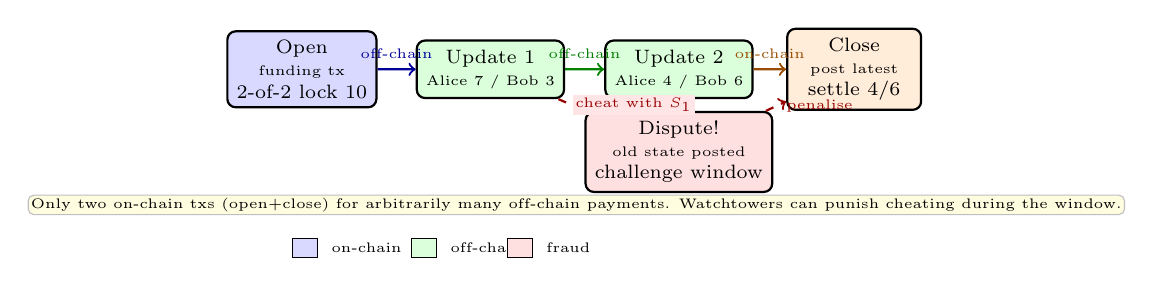
\begin{tikzpicture}[scale=0.84, every node/.style={font=\scriptsize},
  st/.style={draw,rounded corners=3pt,minimum width=1.70cm,minimum height=0.65cm,align=center,thick}]
\node[st,fill=blue!15] (open) at (0,2.10) {Open\\ \tiny funding tx\\ 2-of-2 lock 10};
\node[st,fill=green!14] (up1) at (2.85,2.10) {Update 1\\ \tiny Alice 7 / Bob 3};
\node[st,fill=green!14] (up2) at (5.70,2.10) {Update 2\\ \tiny Alice 4 / Bob 6};
\node[st,fill=orange!15] (close) at (8.35,2.10) {Close\\ \tiny post latest\\ settle 4/6};
\draw[->,thick,blue!60!black] (open)--(up1) node[midway,above,font=\tiny] {off-chain};
\draw[->,thick,green!50!black] (up1)--(up2) node[midway,above,font=\tiny] {off-chain};
\draw[->,thick,orange!60!black] (up2)--(close) node[midway,above,font=\tiny] {on-chain};
\node[st,fill=red!12] (disp) at (5.70,0.85) {Dispute!\\ \tiny old state posted\\ challenge window};
\draw[->,thick,red!60!black,dashed] (up1) -- (disp) node[midway,right,font=\tiny,fill=red!10,inner sep=1pt] {cheat with $S_1$};
\draw[->,thick,red!60!black,dashed] (disp) -- (close) node[midway,right,font=\tiny] {penalise};
\node[font=\tiny,fill=yellow!12,draw=gray!50,rounded corners=2pt,inner sep=1pt,align=center] at (4.15,0.05) {Only two on-chain txs (open+close) for arbitrarily many off-chain payments. Watchtowers can punish cheating during the window.};
% legend
\node[draw,fill=blue!15,minimum width=0.32cm,minimum height=0.18cm] at (0.05,-0.60) {}; \node[font=\tiny,anchor=west] at (0.30,-0.60) {on-chain};
\node[draw,fill=green!14,minimum width=0.32cm,minimum height=0.18cm] at (1.85,-0.60) {}; \node[font=\tiny,anchor=west] at (2.10,-0.60) {off-chain};
\node[draw,fill=red!12,minimum width=0.32cm,minimum height=0.18cm] at (3.30,-0.60) {}; \node[font=\tiny,anchor=west] at (3.55,-0.60) {fraud};
\end{tikzpicture}
\caption{Payment channel lifecycle. The funding transaction and the closing transaction are the only on-chain footprints; everything else is instant, free, off-chain. Posting an outdated state can be challenged.}
\label{fig:channel}
\end{figure}

\emph{Hashed Timelock Contracts (HTLCs)} chain channels into a network (Lightning): payment routes atomically across hops, each hop conditional on revealing a preimage $r$ with $H(r)=h$ before timeout, so intermediaries cannot steal.

\begin{lstlisting}[language=Python]
# Channel state updates (teaching)
class Channel:
    def __init__(self, a_bal, b_bal):
        self.states = [(a_bal,b_bal,0)]
        self.closed=False
    def update(self, a_new, b_new):
        assert not self.closed and a_new+b_new==10, "conservation + open"
        self.states.append((a_new,b_new,len(self.states)))
        return self.states[-1]
    def close(self, idx=None):
        # honest close uses latest; dispute may post old idx
        s = self.states[idx] if idx is not None else self.states[-1]
        self.closed=True
        return s
    def challenge(self, posted_idx):
        # if someone posted old state, honest party can post newer
        if posted_idx < len(self.states)-1:
            return ("penalise cheat, reward honest", self.states[-1])
        return ("close ok", self.states[posted_idx])

ch = Channel(5,5)
print(ch.update(7,3)); print(ch.update(4,6))
print("honest close", ch.close())
# Cheat trace
ch2 = Channel(5,5); ch2.update(7,3); ch2.update(4,6)
print("cheat with idx 1:", ch2.challenge(posted_idx=1))
\end{lstlisting}

Channels excel at many small payments between the same parties, but require liquidity lockup and watchtowers.

% ============================================================
\section{Rollups: Execute Off-Chain, Prove On-Chain}\label{sec:rollups}
A rollup runs a layer-2 chain, batches many transactions, and posts to layer-1 either:
\begin{description}[leftmargin=1.2em,style=nextline]
    \item[Optimistic] Post the new state root and assume correct; allow a \emph{challenge window} (e.g., 7 days) where anyone can submit a \emph{fraud proof} showing mis-execution, which reverts the batch.
    \item[ZK (validity)] Post the new state root plus a succinct ZK proof $\pi$ that the transition was correct; layer-1 verifies $\pi$ instantly (no window).
\end{description}
Both must post \emph{data availability} (enough data for anyone to reconstruct layer-2 state) -- otherwise a malicious sequencer could withhold data and freeze funds.

\begin{figure}[h]\centering
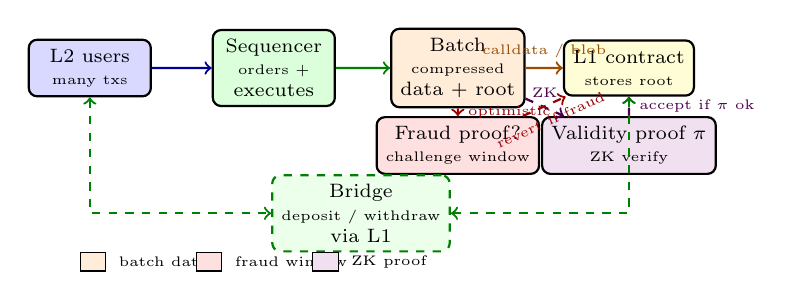
\begin{tikzpicture}[scale=0.82, every node/.style={font=\scriptsize},
  box/.style={draw,rounded corners=3pt,minimum width=1.55cm,minimum height=0.70cm,align=center,thick}]
\node[box,fill=blue!15] (users) at (0,2.35) {L2 users\\ \tiny many txs};
\node[box,fill=green!14] (seq) at (2.85,2.35) {Sequencer\\ \tiny orders +\\ executes};
\node[box,fill=orange!15] (batch) at (5.70,2.35) {Batch\\ \tiny compressed\\ data + root};
\node[box,fill=yellow!16] (l1) at (8.35,2.35) {L1 contract\\ \tiny stores root};
\draw[->,thick,blue!60!black] (users)--(seq); \draw[->,thick,green!50!black] (seq)--(batch); \draw[->,thick,orange!60!black] (batch)--(l1) node[midway,above,font=\tiny] {calldata / blob};
% optimistic path
\node[box,fill=red!12] (fraud) at (5.70,1.15) {Fraud proof?\\ \tiny challenge window};
\node[box,fill=violet!12] (zk) at (8.35,1.15) {Validity proof $\pi$\\ \tiny ZK verify};
\draw[->,thick,red!60!black,dashed] (batch)--(fraud) node[midway,right,font=\tiny] {optimistic};
\draw[->,thick,violet!60!black,dashed] (batch) -- (zk) node[midway,above,font=\tiny] {ZK};
\draw[->,thick,red!60!black,dashed] (fraud)--(l1) node[midway,below,font=\tiny,sloped] {revert if fraud};
\draw[->,thick,violet!60!black,dashed] (zk)--(l1) node[midway,right,font=\tiny] {accept if $\pi$ ok};
% bridge
\node[box,fill=green!8,draw=green!50!black,dashed] (bridge) at (4.20,0.10) {Bridge\\ \tiny deposit / withdraw\\ via L1};
\draw[<->,thick,green!50!black,dashed] (users) |- (bridge); \draw[<->,thick,green!50!black,dashed] (l1) |- (bridge);
% legend
\node[draw,fill=orange!15,minimum width=0.32cm,minimum height=0.18cm] at (0.05,-0.65) {}; \node[font=\tiny,anchor=west] at (0.30,-0.65) {batch data};
\node[draw,fill=red!12,minimum width=0.32cm,minimum height=0.18cm] at (1.85,-0.65) {}; \node[font=\tiny,anchor=west] at (2.10,-0.65) {fraud window};
\node[draw,fill=violet!12,minimum width=0.32cm,minimum height=0.18cm] at (3.65,-0.65) {}; \node[font=\tiny,anchor=west] at (3.90,-0.65) {ZK proof};
\end{tikzpicture}
\caption{Rollup architecture: L2 batches are compressed and anchored on L1. Optimistic rollups rely on fraud proofs within a window; ZK rollups attach a validity proof. Both need a bridge and data availability.}
\label{fig:rollup}
\end{figure}

\begin{lstlisting}[language=Python]
# Rollup batch compression + fraud check (sketch)
import hashlib, json
def compress(txs):  # naive: JSON -> bytes length
    return json.dumps(txs).encode()
def state_root(state): return hashlib.sha256(json.dumps(state,sort_keys=True).encode()).hexdigest()
def apply_batch(state, txs):
    for tx in txs: state[tx["to"]] = state.get(tx["to"],0)+tx["value"]
    return state
# Fraud proof: challenger shows a tx that was misapplied
def verify_fraud(state_before, txs, claimed_root):
    correct = state_root(apply_batch(dict(state_before), txs))
    return correct != claimed_root  # True means fraud proven

s0={"Alice":100}
batch=[{"to":"Bob","value":10},{"to":"Bob","value":5}]
print("compressed", len(compress(batch)), "bytes")
print("correct root", state_root(apply_batch(dict(s0),batch))[:12])
print("fraud?", verify_fraud(s0,batch, "00"*32))
\end{lstlisting}

Trade-offs: optimistic is simpler/EVM-equivalent but withdrawals are slow; ZK is instant but proving is expensive and general EVM ZK is harder.

% ============================================================
\section{Sharding and Data Availability}\label{sec:sharding}
\emph{Sharding} splits validators and state into $k$ shards, each processing a subset of transactions. A beacon chain coordinates cross-shard commits. The hardest problem is \emph{data availability}: how does a light client know a shard's block data was actually published without downloading it all? \emph{Data-availability sampling} (DAS) uses erasure coding plus random spot-checks: if enough random samples are available, the full data is recoverable with high probability.

\begin{figure}[h]\centering
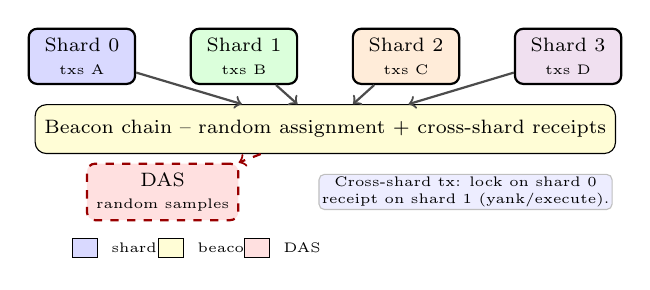
\begin{tikzpicture}[scale=0.84, every node/.style={font=\scriptsize},
  shard/.style={draw,rounded corners=3pt,minimum width=1.35cm,minimum height=0.70cm,align=center,thick}]
\node[shard,fill=blue!15] (s0) at (0,1.85) {Shard 0\\ \tiny txs A};
\node[shard,fill=green!14] (s1) at (2.45,1.85) {Shard 1\\ \tiny txs B};
\node[shard,fill=orange!15] (s2) at (4.90,1.85) {Shard 2\\ \tiny txs C};
\node[shard,fill=violet!12] (s3) at (7.35,1.85) {Shard 3\\ \tiny txs D};
\node[draw,fill=yellow!16,rounded corners=4pt,minimum width=5.2cm,minimum height=0.62cm,align=center] (beacon) at (3.68,0.75) {Beacon chain -- random assignment + cross-shard receipts};
\foreach \s in {s0,s1,s2,s3} \draw[->,thick,gray!60!black] (\s)--(beacon);
\node[shard,fill=red!12,draw=red!60!black,dashed] (sample) at (1.22, -0.20) {DAS\\ \tiny random samples};
\draw[->,thick,red!60!black,dashed] (beacon)--(sample);
\node[font=\tiny,fill=blue!7,draw=gray!50,rounded corners=2pt,inner sep=1pt,align=center] at (5.80,-0.20) {Cross-shard tx: lock on shard 0\\receipt on shard 1 (yank/execute).};
% legend
\node[draw,fill=blue!15,minimum width=0.32cm,minimum height=0.18cm] at (0.05,-1.05) {}; \node[font=\tiny,anchor=west] at (0.30,-1.05) {shard};
\node[draw,fill=yellow!16,minimum width=0.32cm,minimum height=0.18cm] at (1.35,-1.05) {}; \node[font=\tiny,anchor=west] at (1.60,-1.05) {beacon};
\node[draw,fill=red!12,minimum width=0.32cm,minimum height=0.18cm] at (2.65,-1.05) {}; \node[font=\tiny,anchor=west] at (2.90,-1.05) {DAS};
\end{tikzpicture}
\caption{Sharding: execution parallelises across shards coordinated by a beacon chain. Data-availability sampling lets light clients gain confidence without full download. Colour separates per-shard load from coordination.}
\label{fig:sharding}
\end{figure}

Ethereum's post-merge direction is \emph{danksharding} with blobs (EIP-4844): layer-1 provides cheap blob space for rollup data, sharded across validators, rather than full state sharding.

\begin{remark}[Fees and latency across layers]\label{rem:fees-latency}
Channels: instant, near-zero fee, but only between the two participants and require inbound liquidity. Rollups: inherit L1 security, fees are L1 data cost amortised over many L2 txs (often 10--100x cheaper), latency is L2 block time (optimistic withdrawals 7 days, ZK near-instant). Sharding: throughput multiplies with shard count but cross-shard latency adds a round-trip via the beacon. Choosing among them is a latency vs cost vs generality trade-off.
\end{remark}

\begin{example}[Lightning routing]\label{ex:lightning-route}
Alice wants to pay Dave but has no direct channel. She routes via Bob and Carol using HTLCs: each hop locks coins contingent on knowledge of $r$ with $H(r)=h$. Dave, who knows $r$, claims first, revealing $r$ that propagates backwards atomically. If any hop times out, all HTLCs refund -- no intermediary can steal.
\end{example}

\begin{example}[Blob economics]\label{ex:blob}
EIP-4844 introduces blobs that are not executed by L1, only stored for $\sim$18 days and priced separately (blob gas). A rollup posting 120\,KB per batch used to pay $\approx1.9$M gas in calldata; with blobs the same data costs $\approx150$k blob gas -- an order-of-magnitude saving that makes L2 fees sustainable.
\end{example}

% ============================================================
\section{Exercises}\label{sec:ch06-exercises}
\begin{enumerate}[label=E6.\arabic*, leftmargin=*, itemsep=0.6em]
    \item \textbf{Channel math.} Alice and Bob open with 10 coins each. After 100 off-chain payments net is Alice 12 / Bob 8. How many on-chain txs occurred? What happens if Bob posts an old state where he had 15?
    \item \textbf{HTLC route.} Three hops Alice->Bob->Carol->Dave with hash $h=H(r)$. Sketch the lock/unlock order and prove atomicity: Dave reveals $r$ to claim, which lets Carol claim, etc., or all time out.
    \item \textbf{Rollup costs.} A batch of 1000 L2 txs compresses 10x. If L1 calldata costs 16 gas/byte, estimate gas saved vs posting each tx on L1. Repeat for blobs at 1 gas/byte.
    \item \textbf{Optimistic vs ZK.} A new game needs instant withdrawals and full EVM compatibility. Recommend optimistic or ZK and justify with fraud-window vs prover-cost trade-offs.
    \item \textbf{DAS intuition.} A block is erasure-coded into 100 chunks, any 50 recover it. A light client samples 10 random chunks, all available. Bound the probability that $>50\%$ of data is actually withheld.
\end{enumerate}

\section*{Chapter Notes}
Poon--Dryja, Lightning Network (2016) for channels/HTLCs; Buterin, ``A rollup-centric Ethereum roadmap'' (2020) and EIP-4844 for blobs; Gudgeon et al., SoK on layer-2 (2020); Al-Bassam et al., ``Fraud and data availability proofs'' (2019) for DAS; Ethereum danksharding specs (ethereum.org).
% End Ch06
